%%
%% This is file `sample-acmsmall.tex',
%% generated with the docstrip utility.
%%
%% The original source files were:
%%
%% samples.dtx  (with options: `acmsmall')
%% 
%% IMPORTANT NOTICE:
%% 
%% For the copyright see the source file.
%% 
%% Any modified versions of this file must be renamed
%% with new filenames distinct from sample-acmsmall.tex.
%% 
%% For distribution of the original source see the terms
%% for copying and modification in the file samples.dtx.
%% 
%% This generated file may be distributed as long as the
%% original source files, as listed above, are part of the
%% same distribution. (The sources need not necessarily be
%% in the same archive or directory.)
%%
%% Commands for TeXCount
%TC:macro \cite [option:text,text]
%TC:macro \citep [option:text,text]
%TC:macro \citet [option:text,text]
%TC:envir table 0 1
%TC:envir table* 0 1
%TC:envir tabular [ignore] word
%TC:envir displaymath 0 word
%TC:envir math 0 word
%TC:envir comment 0 0
%%
%%
%% The first command in your LaTeX source must be the \documentclass command.
\documentclass[sigplan]{acmart}
%% NOTE that a single column version is required for 
%% submission and peer review. This can be done by changing
%% the \doucmentclass[...]{acmart} in this template to 
%% \documentclass[manuscript,screen]{acmart}
%% 
%% To ensure 100% compatibility, please check the white list of
%% approved LaTeX packages to be used with the Master Article Template at
%% https://www.acm.org/publications/taps/whitelist-of-latex-packages 
%% before creating your document. The white list page provides 
%% information on how to submit additional LaTeX packages for 
%% review and adoption.
%% Fonts used in the template cannot be substituted; margin 
%% adjustments are not allowed.
%%
%% \BibTeX command to typeset BibTeX logo in the docs
\AtBeginDocument{%
  \providecommand\BibTeX{{%
    \normalfont B\kern-0.5em{\scshape i\kern-0.25em b}\kern-0.8em\TeX}}}

%% Rights management information.  This information is sent to you
%% when you complete the rights form.  These commands have SAMPLE
%% values in them; it is your responsibility as an author to replace
%% the commands and values with those provided to you when you
%% complete the rights form.
\setcopyright{acmcopyright}
\copyrightyear{2022}
\acmYear{2022}
\acmDOI{XXXXXXX.XXXXXXX}


%%
%% These commands are for a JOURNAL article.
\acmJournal{JACM}
\acmVolume{37}
\acmNumber{4}
\acmArticle{111}
\acmMonth{8}

%%
%% Submission ID.
%% Use this when submitting an article to a sponsored event. You'll
%% receive a unique submission ID from the organizers
%% of the event, and this ID should be used as the parameter to this command.
%%\acmSubmissionID{123-A56-BU3}

%%
%% The majority of ACM publications use numbered citations and
%% references.  The command \citestyle{authoryear} switches to the
%% "author year" style.
%%
%% If you are preparing content for an event
%% sponsored by ACM SIGGRAPH, you must use the "author year" style of
%% citations and references.
%% Uncommenting
%% the next command will enable that style.
%%\citestyle{acmauthoryear}

%%
%% Personal package imports
\usepackage{listings}
\usepackage{multirow}

% TODO: remove me
\usepackage{todonotes}
\setuptodonotes{inline}

%%
%% end of the preamble, start of the body of the document source.
\begin{document}

%%
%% The "title" command has an optional parameter,
%% allowing the author to define a "short title" to be used in page headers.
\title[Orchestrating the Void]{Orchestrating the Void: Running bespoke applications in empty namespaces on Linux}

%%
%% The "author" command and its associated commands are used to define
%% the authors and their affiliations.
%% Of note is the shared affiliation of the first two authors, and the
%% "authornote" and "authornotemark" commands
%% used to denote shared contribution to the research.
\author{Jake Hillion}
\affiliation{%
  \institution{University of Cambridge}
}
\email{jake.hillion@cl.cam.ac.uk}

%%
%% By default, the full list of authors will be used in the page
%% headers. Often, this list is too long, and will overlap
%% other information printed in the page headers. This command allows
%% the author to define a more concise list
%% of authors' names for this purpose.
%\renewcommand{\shortauthors}{Hillion}

%%
%% The abstract is a short summary of the work to be presented in the
%% article.
\begin{abstract}
  Operating systems are providing more facilities for process isolation than ever before, realised in technologies such as Containers [CN] and systemd slices [CN]. These systems separate the design of the program from the systems that create privilege separation.
  
  Multi-Entrypoint Applications bring the privilege separation back into the program itself. By using a trusted  shim and binfmt\_misc [CN], an application started with minimal privileges can achieve full separation. High-level language features provide an easy interface to privilege separation.
  
  I present a summary of the privilege separation features in modern Linux, the system design of multi-entrypoint applications, the language front-ends to support it, and an evaluation on a series of example applications. 
\end{abstract}

%%
%% The code below is generated by the tool at http://dl.acm.org/ccs.cfm.
%% Please copy and paste the code instead of the example below.
%%
\begin{CCSXML}
<ccs2012>
 <concept>
  <concept_id>10010520.10010553.10010562</concept_id>
  <concept_desc>Computer systems organization~Embedded systems</concept_desc>
  <concept_significance>500</concept_significance>
 </concept>
 <concept>
  <concept_id>10010520.10010575.10010755</concept_id>
  <concept_desc>Computer systems organization~Redundancy</concept_desc>
  <concept_significance>300</concept_significance>
 </concept>
 <concept>
  <concept_id>10010520.10010553.10010554</concept_id>
  <concept_desc>Computer systems organization~Robotics</concept_desc>
  <concept_significance>100</concept_significance>
 </concept>
 <concept>
  <concept_id>10003033.10003083.10003095</concept_id>
  <concept_desc>Networks~Network reliability</concept_desc>
  <concept_significance>100</concept_significance>
 </concept>
</ccs2012>
\end{CCSXML}

\ccsdesc[500]{Computer systems organization~Embedded systems}
\ccsdesc[300]{Computer systems organization~Redundancy}
\ccsdesc{Computer systems organization~Robotics}
\ccsdesc[100]{Networks~Network reliability}

%%
%% Keywords. The author(s) should pick words that accurately describe
%% the work being presented. Separate the keywords with commas.
\keywords{datasets, neural networks, gaze detection, text tagging}


%%
%% This command processes the author and affiliation and title
%% information and builds the first part of the formatted document.
\maketitle

\section{Introduction}

\todo{Write introduction}

\section{Motivation}

\todo{Write motivation}

\subsection{Threat Model}

I present a threat model in which application binaries are trusted absolutely. That is, the software provider had no ill intent, and once the binary is on disk, it will not change without permission. This means that one can trust the binary to set up its own security, as it is protecting not against malice by its own developers, but instead bugs in the software.

\todo{Finalise threat model}

\section{Background}

\subsection{Mount Namespaces}

\section{System Design}

\begin{figure}
    \centering
    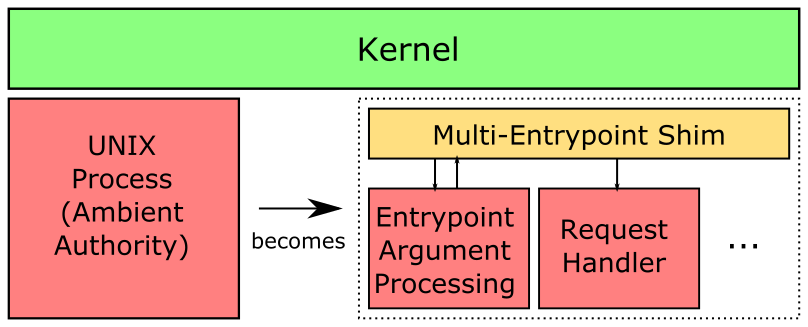
\includegraphics[width=\columnwidth]{figures/self-compartmentalisation-interactions.png}
    \caption{Interaction between the application and the environment.}
    \label{fig:self-compartmentalisation-interactions}
\end{figure}

An example of running a multi-entrypoint application is given in Figure \ref{fig:self-compartmentalisation-interactions}. What was originally a monolithic application becomes a set of applications that communicate with a new shim. The shim does not replace the kernel, and instead supplements it with new higher-level abilities. Each entrypoint receives input from the shim, and can return data to the shim where appropriate. Most of this data is in the form of file descriptors, which are treated as capabilities in this system.

A multi-entrypoint application stores the requirements for running it as static data in the ELF of the binary. When launched, \texttt{binfmt\_misc} is used to launch the application with the multi-entrypoint shim. The shim decodes this data and sets up processes and IPC accordingly.

The shim takes advantage of high levels of privilege to be able to more effectively deprivilege an application than an application with ambient authority could. For example, creating a new network namespace requires \texttt{CAP\_SYS\_ADMIN}, which would give many applications more privilege than they require. By deferring to a shim with extra privileges, this trusted code can be written only once, and avoid conferring more privileges than otherwise required.

\subsection{Building the Void}

Preparing a void for a new process takes advantage of the namespaces feature in Linux. However, many of the namespaces are not designed for this purpose, so this is a more difficult prospect than one might hope. Details of when each namespace was added and some of the relevant features are given in Table \ref{tab:namespaces}.

\begin{table*}
    \centering
    \begin{tabular}{c|c|c}
        Namespace & Date & Kernel Version \\
        \hline
        \texttt{cgroup}   & Fri, 18 Mar 2016 15:09:19 -0400 \citep{heo_git_2016} & v4.6 \citep{torvalds_linux_2016} \\

        \texttt{uts}      & 2006-10-02 02:18:17 -0700 & \\

        \texttt{ipc}      & &\\

        \texttt{network}  & &\\

        \texttt{mount}    & &\\

        \texttt{pid}      & &\\

        \texttt{time}     & &\\

        \texttt{user}     & &
    \end{tabular}
    \caption{Table showing the date and kernel version each namespace was added.}
    \label{tab:namespaces}
\end{table*}

\subsubsection{Mount namespaces}

Mount namespaces were the first [CN] namespaces introduced to Linux, in kernel version X.Y.Z [CN]. In contrast to network namespaces, the API is particularly unfriendly to creating a Void. The creation of mount namespaces is copy-on-write, and many filesystems are mounted shared. This means that they propagate changes back through namespace boundaries. As the mount namespace does not allow for creating an entirely new root, extra care must be taken in separating processes. The method taken in this system is mounting a new \texttt{tmpfs} file system in a new namespace, which doesn't propagate to the parent, and using the \texttt{pivot\_root(8)} tool to make this the new root. By pivoting to the \texttt{tmpfs} without bind mounting the old root inside, the old root becomes completely inaccessible from the namespace. Similarly, the \texttt{tmpfs} never appears in the parent namespace.

\subsubsection{Network namespaces}

Network namespaces are a relatively recent namespace, added in kernel version X.Y.Z [CN]. They present the optimal namespace for creating a void. Creating a new network namespace immediately creates an entirely empty namespace. That is, the new network namespace has no link whatsoever to the creating network namespace. To add a link, one can create a virtual Ethernet pair, with one adapter in each namespace [CN]. Alternatively, one can create a Wireguard adapter with sending and receiving sockets in one namespace and the VPN adapter in another \citep[§7.3]{donenfeld_wireguard_2017}. This allows for very high levels of separation while still maintaining access to the primary resource - the Internet or wider network.

\subsubsection{Remaining namespaces}

\todo{Finish section on remaining namespaces}

\subsection{Something from nothing}

Once a void has been created the goal is to reinsert just enough to run the application, and no more. To allow for running applications in the void with minimal kernel changes, this is done using a mixture of file-descriptor capabilities and adding elements to the namespaces. Capabilities allow for a clean experience where suitable, while adding elements to namespaces creates a more Linux-like experience for the application.

\subsubsection{Files and directories}

\todo{Write section on growing from a void namespace}

\section{Language Frontends}

The language frontends are an extremely important part of this project, closing the gap between a static privilege separation solution like SELinux [CN] and a dynamic one like Capsicum \citep{watson_capsicum_2010}. I have implemented a language frontend in Rust and will describe it in this section.

\subsection{Rust}

\lstset{language=C,caption={A sample application using the Rust language frontend.},label={lst:rust-language-frontend}}
\begin{lstlisting}[float]
#[entrypoint]
fn encrypt(mut in: File, mut out: File)

#[entrypoint]
fn main() {
  let input_file = ...;
  let output_file = ...;
  
  encrypt(input_file, output_file);
}
\end{lstlisting}

The Rust frontend uses macros to wrap functions with high-level primitives into multi-entrypoint compatible entrypoints. Further, it allows calling these functions using the new interface via the shim. Consider the example in Listing \ref{lst:rust-language-frontend}.

Firstly, the encrypt entrypoint is created. This is a regular Rust function which takes two high-level File objects, a wrapped file descriptor. The entrypoint macro wraps this function, providing in its place an \texttt{extern "C"} function that is unmangled and takes argc/argv. This allows functions with high-level arguments to be used as normal, with the argument parsing abstracted away by the library.

Second is the ordinary main function for the application. This is also tagged as an entrypoint, allowing the library to help out with more calls. The example given here is that of the encrypt method, which uses the API seen above. The use of macros here allows the call to encrypt to remain type safe, even though the call must pass through an external interface (the shim itself).

A significant benefit to this approach is the ease of disabling the multi-entrypoint application. By turning the entrypoint macro into identity with a crate feature, the code is compiled without the aid of the multi-entrypoint shim. This allows for significantly easier debugging, as the application follows a single execution path, rather than needing to be debugged as a distributed application.

\section{Example Applications}

\subsection{No Permissions}

The cornerstone of strong process separation is an application that is completely deprivileged. Listing \ref{lst:deprivileged-application} shows an application which, when run under the shim, drops all privileges except \texttt{stdout}. This is easy to achieve under the shim.

\lstset{language=C,caption={An application that requires only stdout and stderr.},label={lst:deprivileged-application}}
\begin{lstlisting}[float]
#[entrypoint(stdout)]
fn main() { println!("hello world!"); }
\end{lstlisting}

\subsection{gzip}

GNU gzip \citep{gailly_gzip_2020} is well structured for privilege separation, though doesn't implement it by default. There is a clear split between the processing logic, selecting the items to do work on, and the compression/decompression routines, each of which are handed a pair of input and output file descriptors. This is shown by Watson et al. in \cite{watson_capsicum_2010}.

As C does not have high-level language features for multi-entrypoint applications, adapting it is slightly more verbose than the other examples seen. However, the resulting code change is still only X lines, if a bit more intricate. This places the risky compression and decompression routines in full sandboxes, while still allowing the simpler argument processing code ambient authority. The argument processing code needs no additional Linux capabilities to manage this permissioning, as the required capabilities are provided by the shim.

\subsection{TLS Server}

\begin{figure}
    \centering
    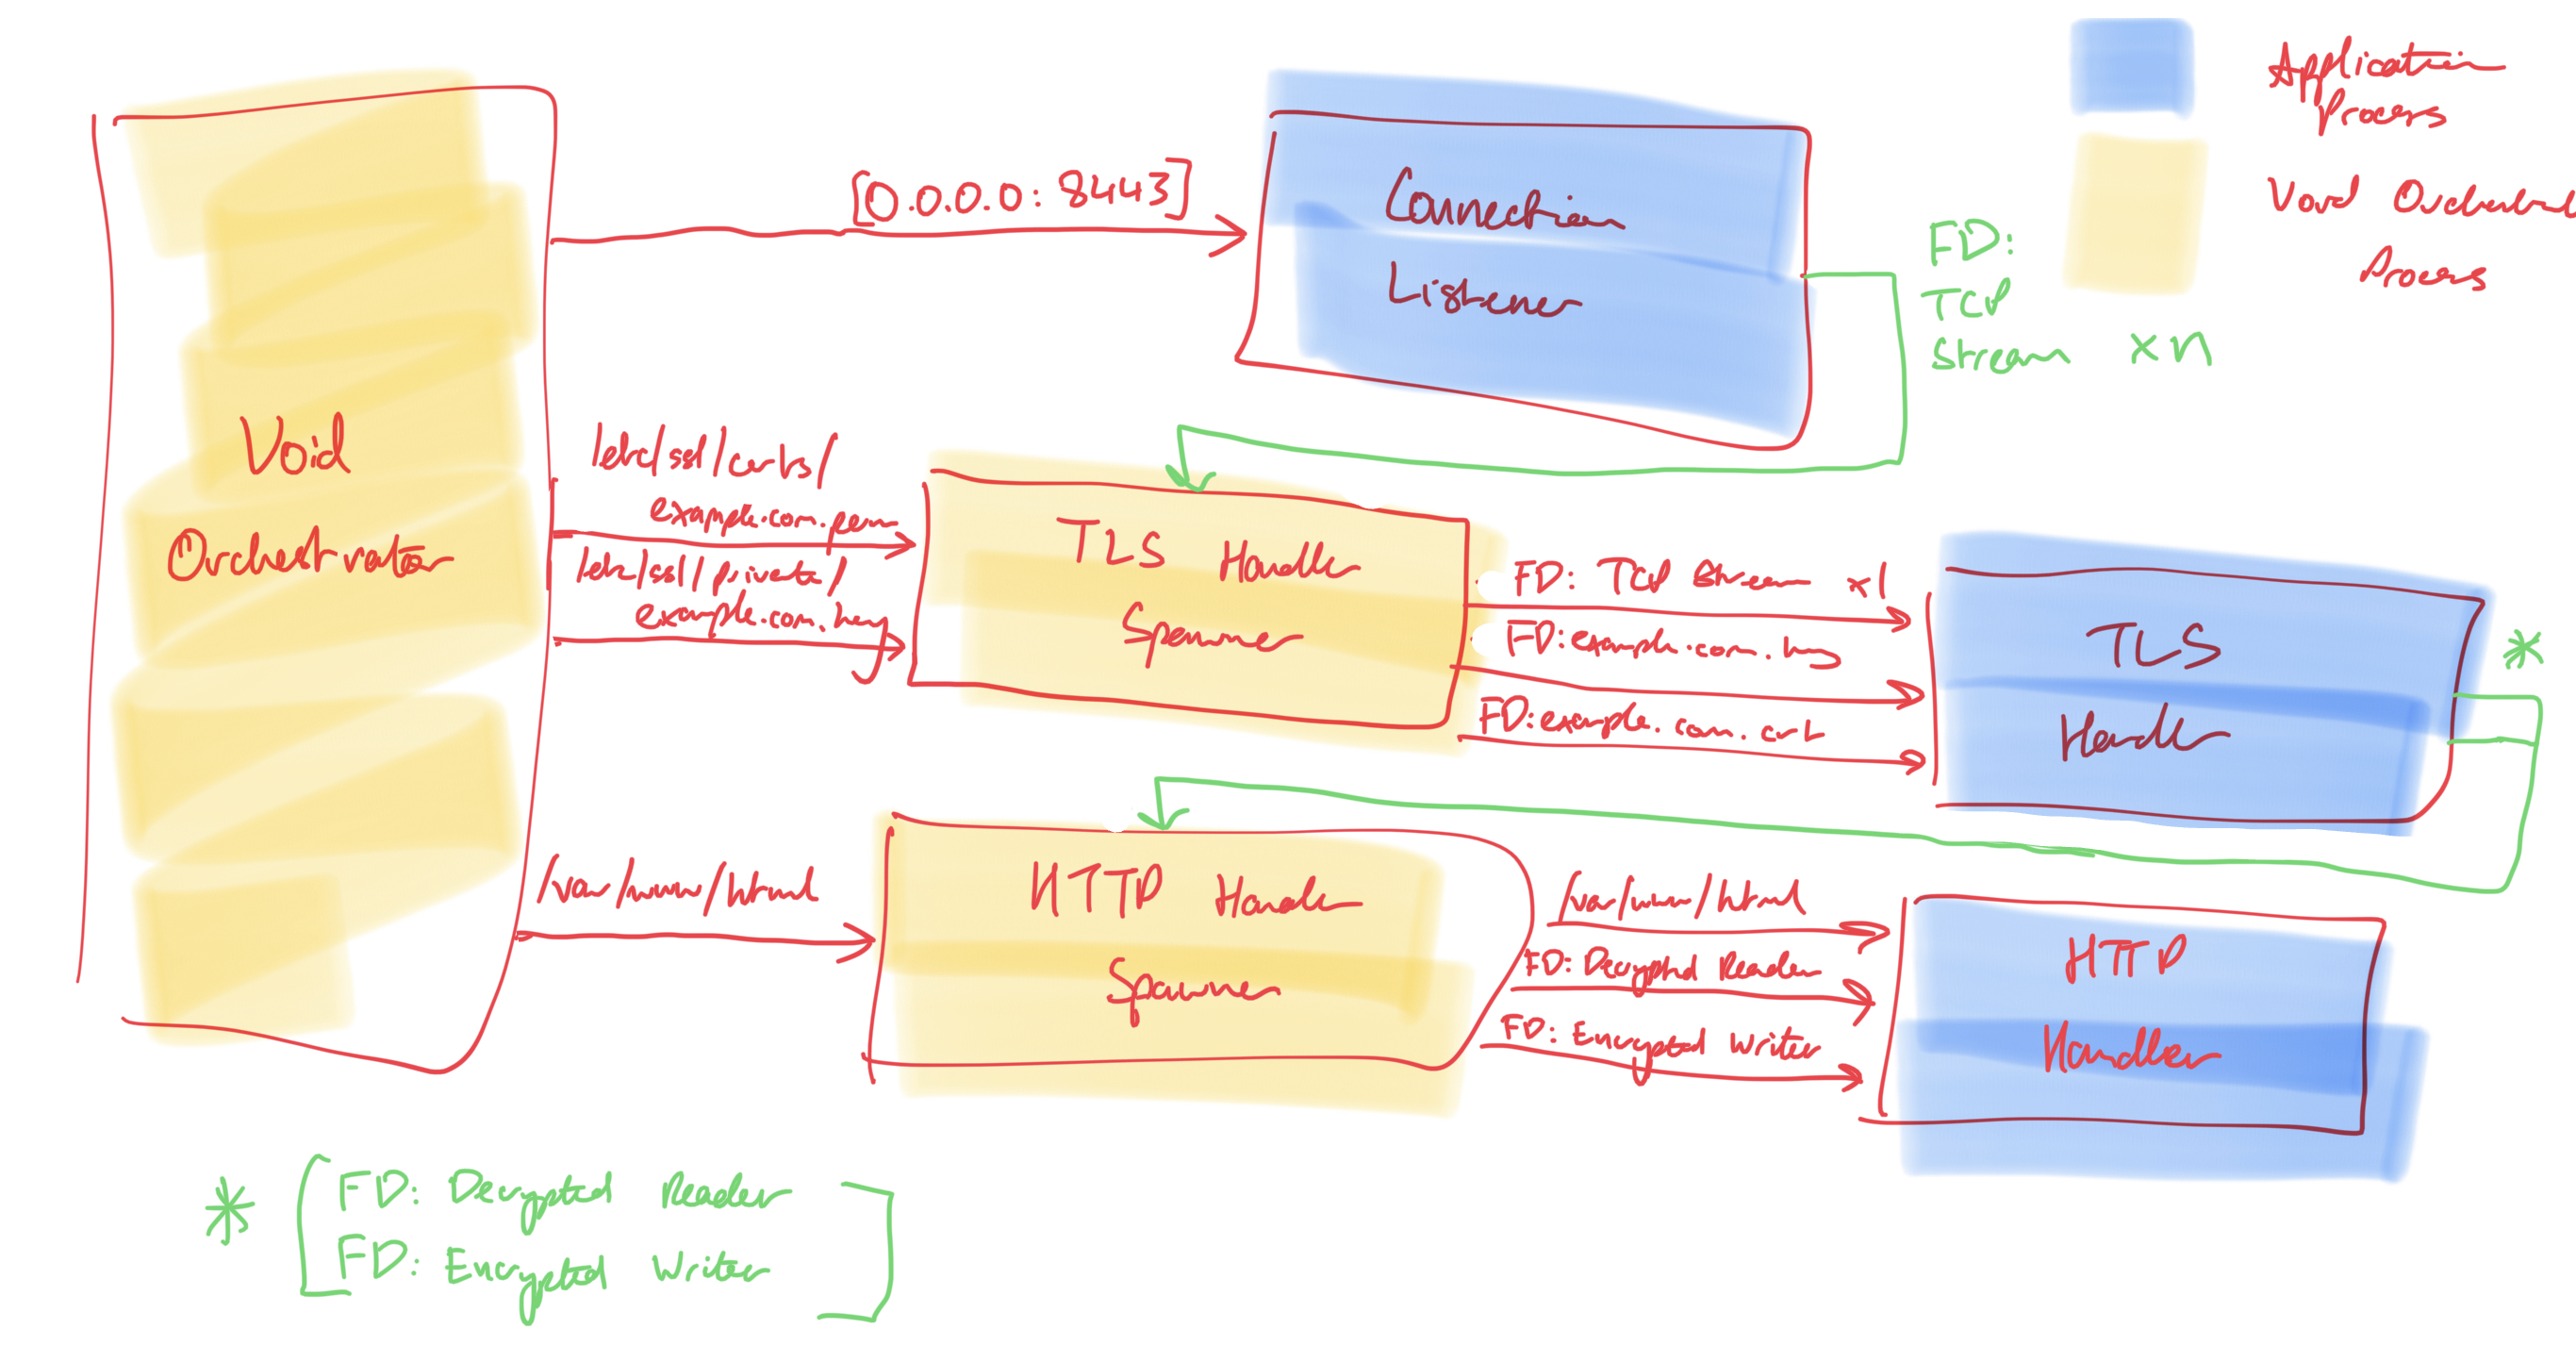
\includegraphics[width=\columnwidth]{figures/tls-server-splitting.png}
    \caption{Process separation in a TLS server.}
    \label{fig:tls-server-splitting}
\end{figure}

Finally, a rudimentary TLS server is created to show the rich privilege separation abilities of multi-entrypoint applications. An example structure is shown in Figure \ref{fig:tls-server-splitting}. Rather than being provided with a view of the network, the initial TCP handling process is given an already bound socket listener by the shim. This allows the TCP handler to live in an extremely restricted zero-access network namespace, while still performing the tasks of receiving new TCP connections.

Next, the TCP handler hands off the new TCP connections to the shim. Though the figure shows this as a direct connection between the TCP handler and the TLS handler, they are passed through the shim, from which the shim spawns a fresh TLS handler for each connection. The TLS handler is handed file descriptors to the certificate and key files that it requires, and hands back a decrypted request reader and an empty response writer file descriptor to the shim.

Finally, this pair of decrypted request reader and response writer are handed to a new process which handles the request. In the example case, this new process is handed a dirfd to \texttt{/var/www/html}, which is bind-mounted into an empty file system namespace by the shim. This allows the request handler enough access to serve files, while restricting access to anything else.

\section{Evaluation}

\todo{Write evaluation}

\section{Related Work}

\subsection{Virtual Machines and Containers}

Virtual Machine solutions \citep{barham_xen_2003,vmware_inc_understanding_2008} provide the ability to split a single machine into multiple virtual machines. When placing a single application in each virtual machine, they are effectively isolated from one another. Full fat container solutions such as Docker [CN], containerd [CN], and systemd-nspawn [CN] provide mechanisms to isolate an application almost completely from other applications running on a single machine. Some have claimed that this provides isolation superior to virtual machines \citep{soltesz_container-based_2007}.

Both of these solutions are less effective at isolating parts of an application from itself [CN with research]. Consider running only a TLS web server in a virtual machine. Although other applications will be unable to access the certificates, as they are in different virtual machines, methods within the application that should not be able to access the certificates still can.

While virtual machines and containers provide a strong isolation at the application level, they are not a compelling solution to intra-application privilege separation.

\subsection{systemd}

\texttt{systemd} [CN] provides a declarative interface to all of the process separation techniques used in this work. Rather than the responsibility of the programmer, creating these declarative descriptions is most commonly left to the package maintainers. This work seeks to provide similar capabilities to the people best suited to privilege separating an application: the developers.

\subsection{Capsicum}

Capsicum \citep{watson_capsicum_2010} extends UNIX file descriptors in FreeBSD to reflect the rights on the object they hold. These capabilities may be shared between processes as other file descriptors (§\ref{section:file-descriptor-passing}). The goals of both software are the same: make privilege separated software better. However, we take quite different approaches. Multi-entrypoint applications focus on building a static definition really close to the code, while Capsicum allows processes to dynamically privilege separate. This allows applying static analysis to the policies, while also keeping the definition close to the code.

\section{Future Work}

\subsection{Dynamic Linking}

\todo{Write section on dynamic linking future work}

\section{Conclusion}

\todo{Write conclusion}

%%
%% The acknowledgments section is defined using the "acks" environment
%% (and NOT an unnumbered section). This ensures the proper
%% identification of the section in the article metadata, and the
%% consistent spelling of the heading.
\begin{acks}
\todo{Write acknowledgements}
\end{acks}

%%
%% The next two lines define the bibliography style to be used, and
%% the bibliography file.
\bibliographystyle{ACM-Reference-Format}
\bibliography{references}

%%
%% If your work has an appendix, this is the place to put it.
\appendix

\end{document}
\endinput
%%
%% End of file `sample-acmsmall.tex'.
